\section{Approach}
\label{sec:approach}
Since there are no reference summaries for training,
we design a weakly supervised approach, 
which first synthesizes the semi-structured training data and 
then provides an aspect-guided summarization model for semi-structured data.

\subsection{Semi-structured Training Data Creation}
\label{sec:data}
Let $R$ denote the set of all reviews about entity $e$.
To avoid information loss in textual inputs or structured inputs,
we create a synthetic semi-structured training dataset %$\mathbb{D}$ 
with four steps, 
as shown in \figref{fig:dm}:
(1) \textbf{sample a review} $r_s$ as a summary from $R$ and take $R - \{r_s\}$ as candidate reviews $R'$; 
(2) \textbf{extract opinion-aspect pairs (OAs) and implicit sentences (ISs)} from $R'$ and $r_s$;
suppose that $O'$ is OAs extracted from $R'$ and
$I'$ is ISs from $R'$, 
(3) {\bf sample} some {\em matched OAs} and {\em mismatched OAs} from $O'$ to act as \textbf{noisy OAs} according to the OAs in $r_s$;
and (4) {\bf sample} a subset of ISs from $I'$ to act as \textbf{noisy ISs} according to the ISs in $r_s$. 
The noisy OAs and noisy ISs simulate the OAs and ISs in the actual multi-review that do not show up in the sampled summary $r_s$.
We give more details of these four steps next.

\begin{figure}[th]
	\centering
	\includegraphics[width=1.0\linewidth]{./dm.pdf}
	\caption{Semi-structured training data creation.  
The semi-structured training data consists of semi-structured input and textual output pairs. (1)\textasciitilde(4) correspond to the four steps of creating data in first paragraph of \secref{sec:data}.}
	\label{fig:dm}
\end{figure}

\subsubsection{Summary Sampling.} 
To sample summary $r_s$,
we ignore the reviews containing first-person singular pronouns
and non-alphanumeric symbols except punctuation~\cite{Denoise20},
since such reviews don't look like real summaries.
Besides, we ensure that all aspects of the summary can be found in $R'$.
This stems from the fact that aspects in a summary should not come  
from outside of its multi-review.

\subsubsection{Opinion-aspect Pairs and Implicit Sentences Extraction.} 
We follow \citet{sampo} to extract opinion-aspect pairs
\footnote{Our framework is not specific to any opinion-aspect extraction algorithm or tool.            
We choose to use \cite{sampo} because it is an unsupervised method, 
which is better at creating synthetic datasets for cross-domain review corpora (i.e., product, service or movie).}, 
which first utilizes MIN-MINER~\cite{basicOpiMin20} to 
get the dependency parse trees of the sentences first and then uses a set of 
syntactic rules~\cite{aspect12} to extract OAs
 \footnote{https://github.com/sampoauthors/Sampo}, 
i.e., (opinion, aspect) pairs.
Meanwhile, we collect those sentences from which no OAs were extracted, and call these sentences ISs. 
As shown in \tabref{tab:ours_data}, the semi-structured output contains the OAs and ISs extracted from 
its textual output.

Given a review $r$, the OAs extracted from $r$ have different aspects.
For an aspect $a$,
let $O_a$ as the set of OAs based on $a$. 
We take $o$ as an OA pair in $O_a$
and $f$ as the number of occurrences of $o$.
We extract OAs and ISs from sampled summary $r_s$
and candidate reviews $R'$.
The extracted OAs in $R'$ is indicated as $O'$.
For an aspect $a$ in summary,
the set of OAs with the same aspect in $O'$ is represented as $O'_a$.%$=\{(o'_{1}, f'_1), ..., (o'_{N}, f'_{n'})\}$. 
The definition of $o'$ and $f'$%, and $n'$
are similar to $o$ and $f$, except that they refer to the ones in $O'_a$.
The set of ISs in $R'$ is represented as $I'$.

\subsubsection{Noisy Opinion-Aspect Pairs Sampling}
%In actual multi-review and summary pairs, 
%the aspects mentioned in a summary 
%should be a subset of aspects in multi-review.
Actual multi-review is the noisy version of its summary,
which includes all aspects in the summary and some aspects that are not in the summary.
%which has both the same and different aspects as the summary.
To simulate actual multi-review, 
there are two types of noisy OAs: 
{\em matched} (MA) OAs and {\em mismatched} (MM) OAs.
The OAs with the same aspects as summary are MA,
and the others OAs are MM.
For example, suppose that (disappointed, food) is an OA in summary,
(bad, food) is an MA pair and (not fresh, beef) is an MM pair.

To obtain noisy MA OAs, 
we sample some matched OAs from $O'$ for each aspect in summary and collect the sampled OAs together.
In some actual multi-reviews, some people may have inconsistent comments on the same aspect of an entity.
So we sample noisy MA OAs by
the distribution of cosine similarity
between OAs with the same aspects in $O'$ and summary,
which can get a few OAs with conflict opinions like OAs in normal multiple reviews.
To compute similarity,
we take each OA as a sequence of tokens in its opinion and aspect.
We use GloVe~\cite{glove}
\footnote{https://nlp.stanford.edu/projects/glove/}
to represent tokens
and take the average of embeddings of the tokens in sequential OA
as {\em OA embedding}.
Suppose $a$ is an aspect of OAs in the sampled summary, 
$O'_a$ is composed of all matched OAs based on aspect $a$ in $O'$.
$\boldsymbol{o_s}$ is the vector representing all OAs on $a$ in summary, 
which is the average of the corresponding OA embeddings.
We compute the cosine similarity score between $\boldsymbol{o}$ and a matched OA pair $o'$ in $O'_a$ as: $cs(a)=cosine\_sim(\boldsymbol{o'}, \boldsymbol{o_s})$,
where $\boldsymbol{o'}$ is the embedding of $o'$.
$\mathbf{cs}(a)$ consists of the cosine similarity scores 
of all matched OA pairs on $a$.
We normalize the cosine similarity scores of $a$
by $\mathbf{cs}'(a)=softmax(\mathbf{cs}(a))$. 
The $\mathbf{cs}'(a)$ denotes the probability distribution 
%of OAs in a matched aspect.
of all matched OAs on aspect $a$.
Then, we sample $N_{ma}$ matched OAs on aspect $a$ according to the distribution $\mathbf{cs'}(a)$. 

To obtain noisy MM OAs, 
we randomly sample $N_{mm}$ mismatched OAs from $O'$,
which satisfies the randomness
of OAs that appear in actual multi-review 
and not in its summary.
%$N_{mm}$ is the number of mismatched OAs that should be sampled.

%To make the number of sampled matched OAs and mismatched OAs closer to actual multi-review,
As the number of OAs based on different aspects in multiple reviews of the same entity is not identical,
$N_{ma}$ should be sampled by the distribution of 
the number of matched OAs
between actual multi-review and its summary.
Because there are no actual multi-review and summary pairs,
we randomly extract $N_r$ reviews from each entity
as a {\em pseudo-multi-review}, and suppose that the aspects appearing in more than one review are MA aspects
and others are MM aspects.
$N_r$ is a constant.
In this way, for each aspect in sampled summary, 
$N_{ma}$ is sampled as:
\begin{equation}
N_{ma} \sim Gaussian(\mu_{ma}, \sigma_{ma}^2),
\end{equation}
where $\mu_{ma}$ and $\sigma_{ma}$ are the mean and standard deviation of
the number of matched OAs on different aspects 
in the set of {\em pseudo-multi-reviews}.
Similarly, we get
$N_{mm} \sim Gaussian(\mu_{mm}, \sigma_{mm}^2)$ 
for noisy MM OAs.
$\mu_{mm}$ and $\sigma_{mm}$ are the mean and standard deviation of
the number of mismatched OAs in different {\em pseudo-multi-reviews}.
Sampled matched OAs and mismatched OAs compose noisy OAs.

\subsubsection{Noisy Implicit Sentences Sampling.}
Given a sampled summary $r_s$, 
we compute the ROUGE-1 recall score between the set of the ISs in $r_s$
and each sentence in $I'$.
We get the probabilities of sentences in $I'$
by the $softmax$ function on their R-1 recall scores. 
We sample $N_{I}$ sentences from $I'$ by
the probability distribution:
$N_{I} \sim Gaussian(\mu_{I}, \sigma_{I}^2)$.
$\mu_{I}$ and $\sigma_{I}$ are the mean and standard deviation of 
the number of ISs in {\em pseudo-multi-reviews}.
%For each step, we remove the sampled sentence and recalculate the probability distribution of remained sentences in $I'$.
We collect all the sampled ISs as noisy ISs.


\subsection{Summarization Models}
\label{sec:model}

\cut{%%%%
\begin{figure*}[t]
	\centering
	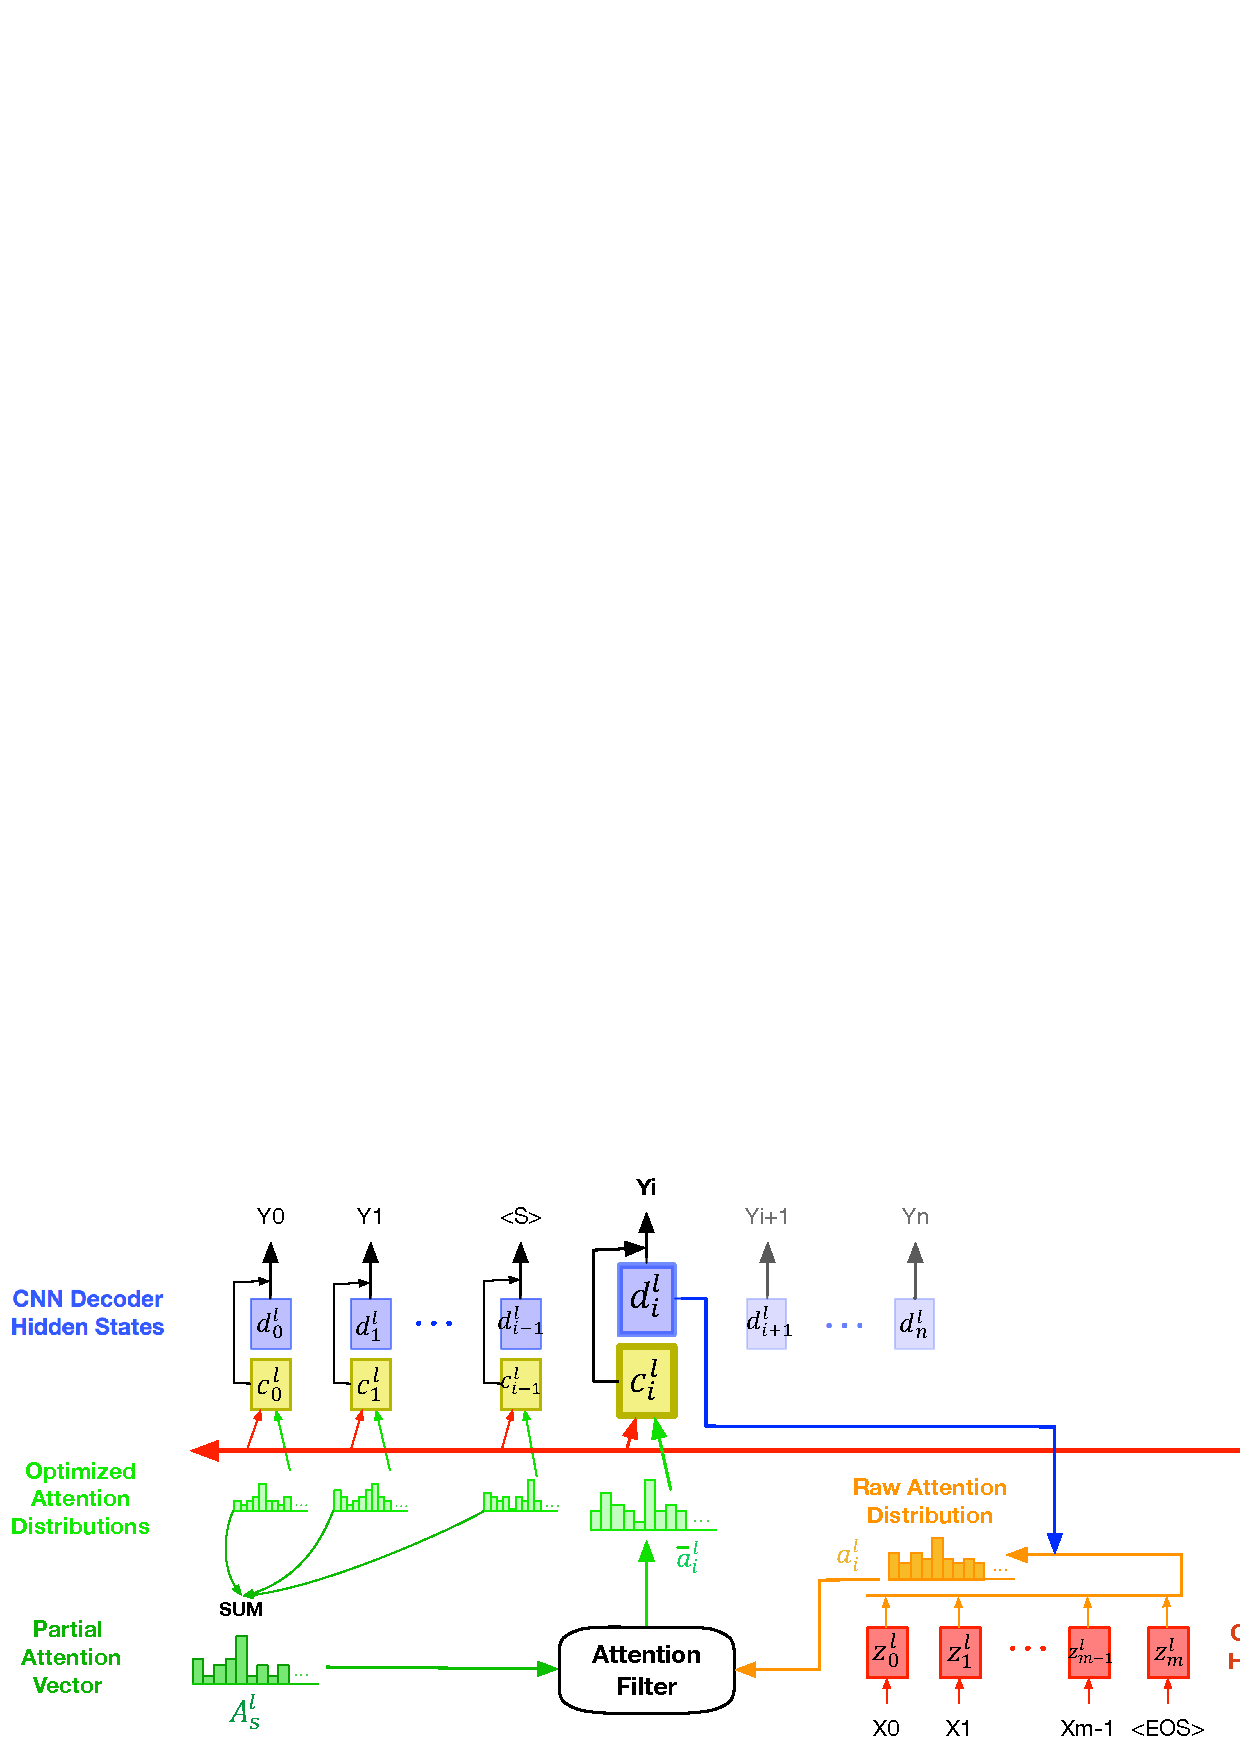
\includegraphics[width=1\linewidth]{./model.pdf}
	\caption{The architecture of AMO and AMD. \KZ{I suggest you break this figure up into two separate narrow figs 
to save some space. Note the (1) and (1) above the figs.}}
	\label{fig:model}
\end{figure*}
}%%%%%

Given noisy OAs and ISs as input, the model should deal with them in different ways 
because OAs and ISs play different roles in generating a summary.
The explicit information of a summary is mainly generated by selecting the key OAs from noisy OAs and 
rephrasing the selected OAs into complete sentences.
Noisy ISs will be used to summarize implicit information.
When generating summaries, 
the explicit information (noisy OAs) and the implicit information (noisy ISs) also interact with each other.

In this subsection, we first present a \textbf{basic aspect-guided model with an encoder} taking only noisy OAs as input, which learns to select accurate aspects and their appropriate opinions 
to generate explicit information.
Then we further propose an {\bf advanced aspect-guided model with a dual encoder} taking both OAs and ISs as input.
In opinion summarization, 
since OAs are the most important information while ISs are supplementary, 
our best approach is to \textbf{train the advanced aspect-guided model initialized with pretrained basic aspect-guided model}.
%In order to get high-quality summaries,

In our models, 
we concatenate the opinion and aspect in each OA.
To model the relation among OAs,
we add a special token at the beginning of each OA, 
which indicates the OA representation.
As there is no order among OAs, 
we concatenate the OAs in noisy OAs in a shuffled order. 
$x^O_{i,j}$ is the $i^{th}$ token of $j^{th}$ OA in noisy OAs ($\textbf{x}^O$). The special token of $j^{th}$ OA is $x^O_{0,j}$.
The sentences in noisy ISs ($\textbf{x}^I$) are concatenated in the
same way as noisy OAs.
$x^I_{0,j}$ is the special token of $j^{th}$ sentence.
We take noisy OAs $\textbf{x}^O$ and noisy ISs $\textbf{x}^I$as input and summary $\textbf{y}$ as output.


\subsubsection{Basic Aspect-guided Model}
We adopt a transformer seq2seq model~\cite{Transformer17} as the basic model,
which has an OA encoder taking only noisy OAs $\textbf{x}^O$ as input.
The basic model is in \figref{fig:amo}.

\begin{figure}[th]
	\centering
	\includegraphics[width=1\linewidth]{./AMO.pdf}
	\caption{The architecture of basic aspect-guided model.}
	\label{fig:amo}
\end{figure}

$\textbf{h}^O$ is the output of encoder.
$c_t$ is the context vector, which is the weighted sum of $\textbf{h}^O$ with Encoder-Decoder Attention (\textbf{{\em Enc-Dec Attn}}) as weight.
After a feed-forward network of transformer~\cite{Transformer17},
$c_t$ becomes $c'_t$.
The probability distribution of 
generating $y_t$ is calculated by:
\begin{equation}
p(y_t|y_0,...,y_{t-1}, \textbf{x}^O)=softmax(W^O c'_{t-1}+b^O),
\label{eq:decode}
\end{equation}
where $W^O$ and $b^O$ are trainable parameters.

The basic model with only noisy OAs as input attends to the important pairs in noisy OAs, 
and consequently tends to generate general and simple summaries.
We thus add implicit opinion by introducing noisy ISs $\textbf{x}^I$ to the model.
	
\subsubsection{Advanced Aspect-guided Model}
We design an advanced model that parallelly deals with noisy OAs and ISs
via two transformer encoders, \textbf{\em OA encoder} and \textbf{\em IS encoder}. 
The parameters of the dual encoder are not shared.
The architecture is illustrated in \figref{fig:amd}.

\begin{figure}[th]
	\centering
	\includegraphics[width=1\linewidth]{./AMD.pdf}
	\caption{The architecture of advanced aspect-guided model. 
}
	\label{fig:amd}
\end{figure}

Inspired by~\citet{DialogMV2020},
%we represent the $j$-th OA pair in the noisy OAs by 
%the latent representation of the $j$-th special token $x^O_{0,j}$.
we use $H^O_{j}$ to denote the encoder hidden state of $x^O_{0,j}$,
which represents the $j^{th}$ OA pair in noisy OAs.
$\textbf{H}^O=\{H^O_{1},...,H^O_n\}$ consists of all special tokens of noisy OAs.
Then, we aggregate the information of all pairs in noisy OAs through self-attention mechanism (\textit{SelfAttn})~\cite{Transformer17}:
\begin{align}
	\alpha_{i,j} &= \frac{\exp(H^O_i H^O_j)}{\sum_{k=1}^{n}\exp(H^O_i H^O_k)}\\
    A^O_{i} &= \sum\nolimits_{j=1}^{n}\alpha_{i,j}  H^O_j \\
    \alpha_{i,j}' &= \frac{\exp(A_i^O)}{\sum_{i=1}^{n}\exp(A_i^O)} \\
    \textbf{A}^O&= \sum\nolimits_{i=1}^{n} \alpha_{i,j}' A^O_i
\end{align}
where $\textbf{A}^O$ denotes the total information of noisy OAs.
Similary, we can get all special tokens of noisy ISs, $\textbf{H}^I$, and the IS representation $\textbf{A}^I$.
The {\em OA probability} $	\widetilde{\lambda}^O$
and 
{\em IS probability} $	\widetilde{\lambda}^I$ are compute as:


\begin{align}
	\widetilde{A}^O &= \tanh(W_1\textbf{A}^O+b_1) \\
	\widetilde{A}^I &= \tanh(W_2\textbf{A}^I+b_2) \\
    \lambda^O &= \frac{\exp(\widetilde{A}^O {^\top} v^O)}{\exp(\widetilde{A}^O {^\top} v^O)+\exp(\widetilde{A}^I {^\top} v^I)}  \\
	\widetilde{\lambda}^O &=\frac{ \lambda^{O\frac{1}{T}}}{\lambda^{O\frac{1}{T}}+(1-\lambda^O)^{\frac{1}{T}}}
	\label{eq:T}  \\
	\widetilde{\lambda}^I &=1-\widetilde{\lambda}^O,
\end{align}
where $v^O$ and $v^I$ respectively denote the randomly initialized context vector of OA encoder and IS encoder.
$W$ and $b$ are parameters. $T$ is the temperature for sharpening the attention distribution between encoders.
At each decoding step $t$, 
$C_t^O$ is the weighted sum of encoder hidden states of OA with \textbf{{\em Enc-Dec Attn}} as weight. 
$C_t^I$ is the weighted sum of IS encoder.
The combinational context vector $C_t$ for decoding is:
%of the Encoder-Decoder Attention 
%is the weighted sum of $C_t^p$ and $C_t^s$ as:
%is computed as:
%The combinational context vector $C_t$ for decoding is:
\begin{equation}
	C_t = \widetilde{\lambda}^O C_t^O +  \widetilde{\lambda}^I C_t^I
\end{equation}
%\KZ{How? $C_t$ should be modified by feed-forward network and becomes $G_t$.} 
We get $C'_t$ by inputting $C_t$ to the feed-forward network layer of transformer \cite{Transformer17}.
The probability distribution of generating $y_t$ is:
\begin{equation}
p(y_t|y_0,...,y_{t-1}, \textbf{x}^O,\textbf{x}^I)=softmax(WC'_{t-1}+b),
\end{equation}
where $W$ and $b$ are the trainable parameters.
%In this model, the decoder hidden state of MAGOS is $\mathbf{Z}=(Z_0,...,Z_T)$. The decoder state at timestep $t+1$ should be calculated from
%$Z_t$ and $C_t$. 
%We also use the $softmax$ function to compute the probability distribution of 
%generation over $\mathbf{Z}$.
%The probability distribution over vocabulary of decoder is the same as Equation \ref{eq:decode}.

\subsubsection{Training Advanced Aspect-guided Model}
\begin{figure}[th]
	\centering
	\includegraphics[width=1\linewidth]{./flow.pdf}
	\caption{Training process of optimizing advanced model. The structures in Step 1 and Step 2 are the simplified version of architectures in \figref{fig:amo} and \figref{fig:amd}, respectively.}
	\label{fig:flow}
\end{figure}

%\KZ{No need to have OAM, just say the way to train the advanced model.}
%\subsubsection{MB}
%\textbf{Optimization: MAI based on BAG (MB)}
For optimization, we first train the basic model to extract and generate the explicit information from noisy OAs ({\bf Step 1} in \figref{fig:flow}).
%Summaries generated by BAG
Then, we further fine-tune the advanced model based on the pretrained
basic model, enhancing the generated summary with
implicit opinion from noisy ISs ({\bf Step 2} in \figref{fig:flow}).
At Step 2, the parameters of OA encoder and the attention between OA encoder and decoder are initialized by pretrained basic model.
%\KZ{I don't see OAM in the fig.} 
%\KZ{Earlier you gave me the impression that BAG, AI and MAI etc, are all alternative
%summarization models that work on the synthetic pairs. But after this section,
%it seems that these models work together as components to a bigger thing?}

%We extract OAs and ISs of multi-review as noisy OAs and noisy ISs,
%which are the input of models.
%The human-written summaries are output.



